\documentclass[KITtoc]{beamer}
\mode<presentation>
{
  \usetheme[english,titlepage0]{KIT}
  %\setbeamercovered{transparent}
  %\setbeamertemplate{enumerate items}[circle]
}

\TitleImage[width=\titleimagewd]{img/KIT-Titel7}

\usepackage{etex}
\usepackage[utf8]{inputenc}
\usepackage[T1]{fontenc}
\usepackage{array}
\usepackage{multicol}
\usepackage{ragged2e}
\usepackage{bbm}
\usepackage{algorithmic}
\usepackage{marvosym}

\usepackage{tikz,pgfplots}
\usetikzlibrary{calc,positioning,arrows,shapes}
\usetikzlibrary{decorations.pathreplacing}

\makeatletter
\def\slot[#1,#2](#3);{{
	\draw  (#3,0) rectangle (#3+0.5,0.5) node[midway] (#2) {#1};
}}
\makeatother

\RequirePackage{xcolor}

\newcommand<>{\galert}[1]{{\color#2{KITgreen}#1}}
\newcommand<>{\balert}[1]{{\color#2{KITblue}#1}}
\newcommand<>{\ralert}[1]{{\color#2{KITred}#1}}

\title[GBD]{\textbf{Collective Management of Benchmark Metadata}}
\subtitle{Markus Iser, Carsten Sinz}
\author[Markus Iser, Carsten Sinz]{Markus Iser, Carsten Sinz}
\institute[Karlsruhe Institute of Technology (KIT)]{KARLSRUHE INSTITUTE OF TECHNOLOGY (KIT)}

\begin{document}

\begin{frame}
\maketitle
\end{frame}

\begin{frame}{Motivation}
\begin{block}{Dealing with large amounts of benchmark data}
\begin{itemize}
\item Distributed over different groups and computers
\item Names are not unique, duplicate benchmark problems
\item Searching for problems with specific properties
\end{itemize}
~\\[.7em]
How do we store properties such that they can be safely assigned to the problem?
\end{block}
\end{frame}

\begin{frame}{Roadmap}
\tableofcontents
\end{frame}

\section{Classes of Benchmark Data}

\begin{frame}{Classes of Benchmark Data}
\begin{block}{Meta-data (non-calculable)}
\begin{itemize}
\item Author
\item Generator
\item Encoding
\item Application Domain
\item Local Path
\item Online Source
\item Inclusion in Competition Set
\item \dots
\end{itemize}
\end{block}
\end{frame}

\begin{frame}{Classes of Benchmark Data}
\begin{block}{Feature-data (calculable, easy)}
\begin{itemize}
\item Number of Variables / Clauses
\item Maximum clause-length
\item Number of connected components
\item Tree-width
\item Problem class (Horn, 2-SAT, etc.)
\item \dots
\end{itemize}
\end{block}
\end{frame}

\begin{frame}{Classes of Benchmark Data}
\begin{block}{Heavyweight Data (calculable, hard)}
\begin{itemize}
\item Solution to SAT-Problem
\item Number of Solutions
\item Isomporphic Problems
\item Size of shortest (recorded) Proof
\item Runtimes
\item Best (recorded) runtime
\item \dots
\end{itemize}
\end{block}
\end{frame}


\section{Metadata Usage}

\begin{frame}{Use Case: Correlation Analysis}
Very common to analyze runtimes with respect to SAT result.\\[2em]
\begin{tabular}{c|cc}
Mixed Result & SAT Result & UNSAT Result \\
\hline
 & & \\
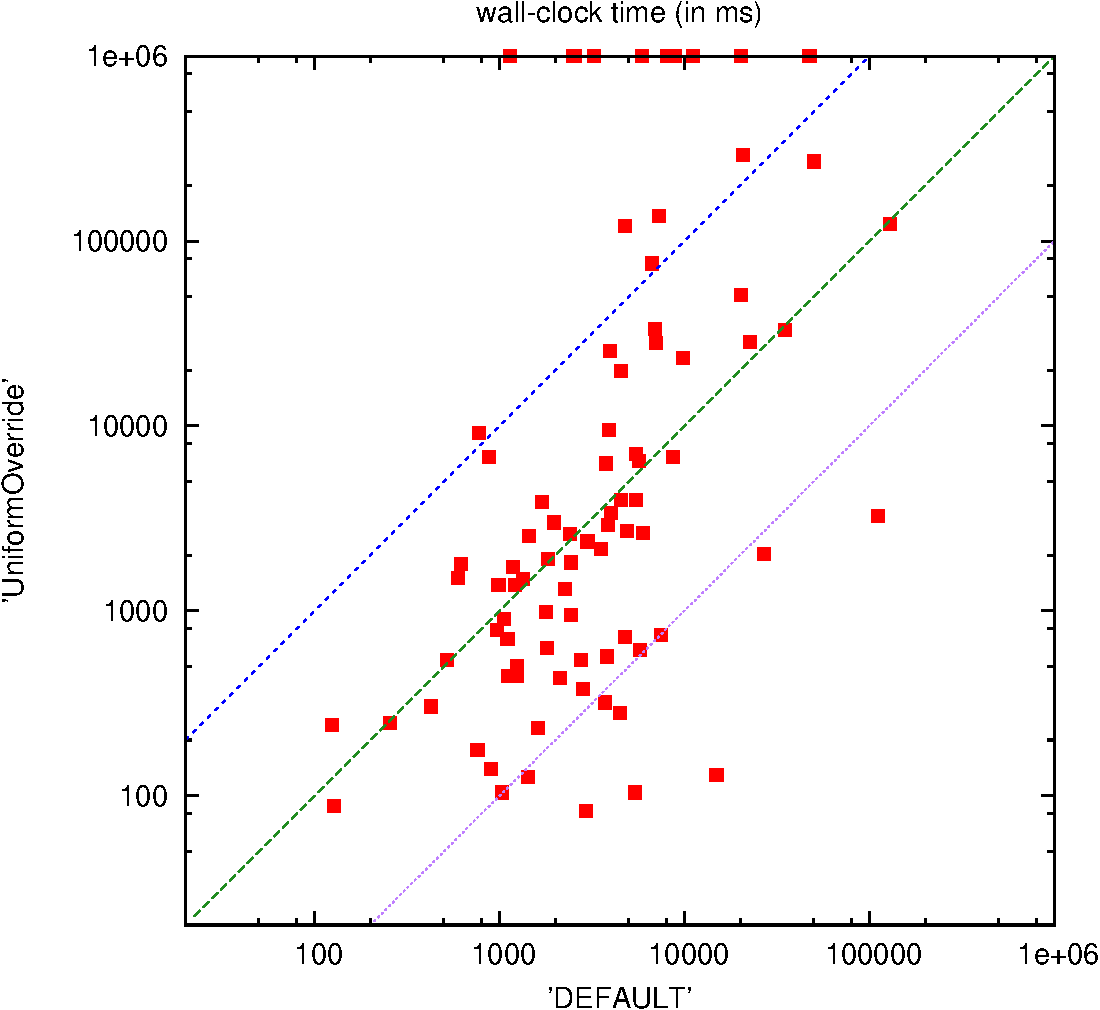
\includegraphics[width=.3\linewidth]{fig/Override.pdf} &
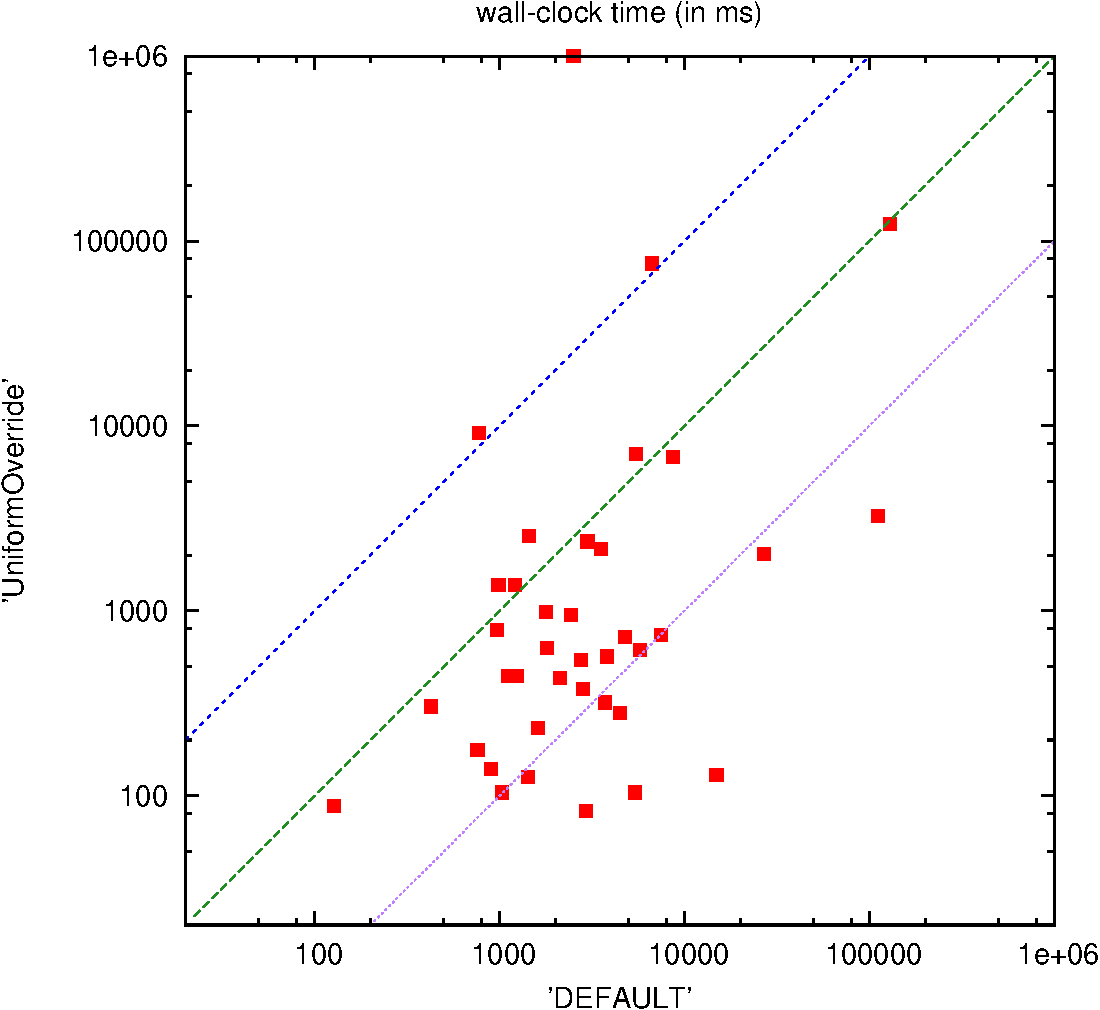
\includegraphics[width=.3\linewidth]{fig/OverrideSAT.pdf} &
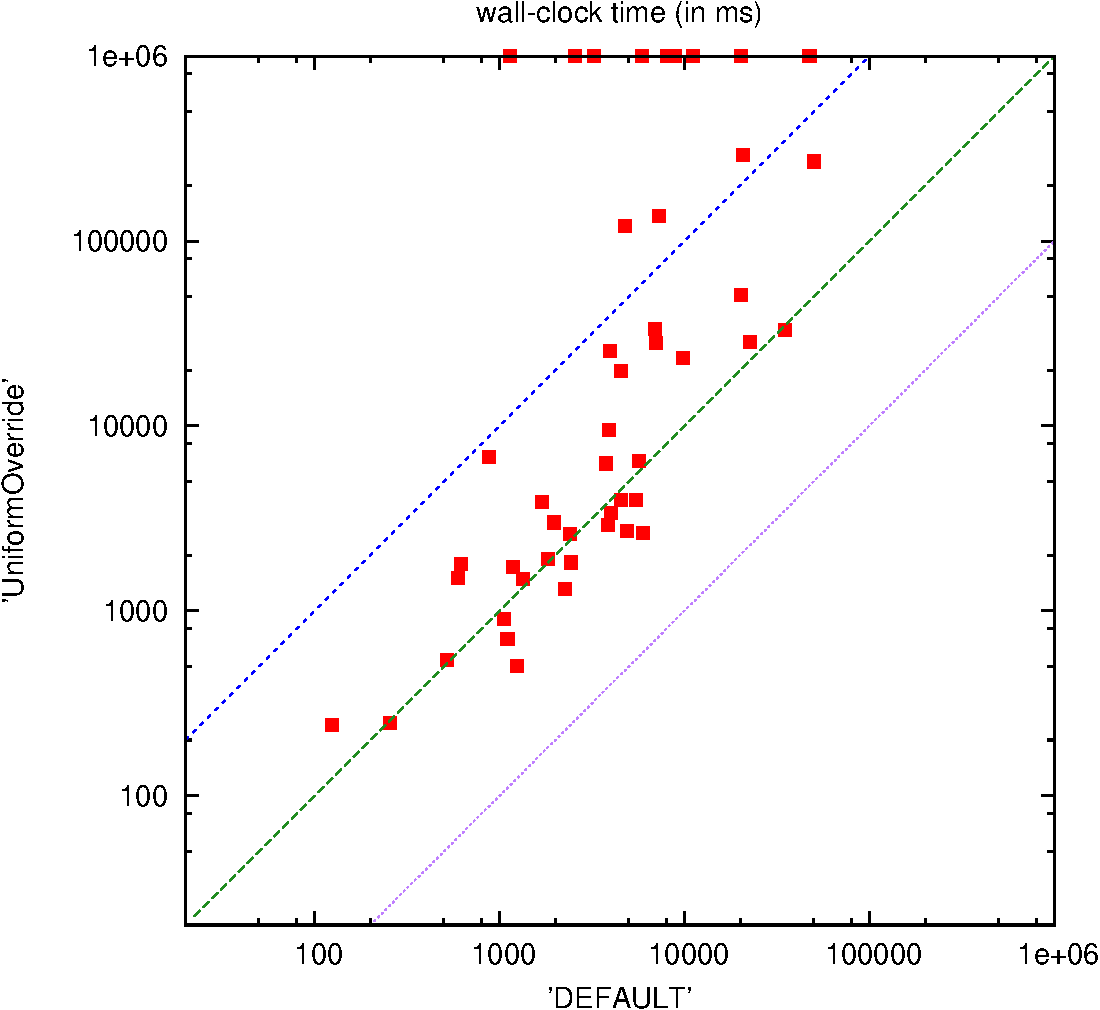
\includegraphics[width=.3\linewidth]{fig/OverrideUNSAT.pdf}
\end{tabular}
\end{frame}

\begin{frame}{Use Cases}
\begin{block}{Correlations}
\begin{itemize}
\item Experimentation $\rightarrow$ Observation $\rightarrow$ Conclusion
\item Come to conclusions with previously ``inconclusive'' results
\item Possibility of correlation-based hypothesis 
\end{itemize}
\end{block}
\begin{block}{Elimination of Duplicate Benchmarks}
\begin{itemize}
\item Clause and Literal Ordering
\item Variable Renaming
\item Create Equivalence Class $\rightarrow$ Choose Representant $\rightarrow$ Union-Find
\end{itemize}
\end{block}
\end{frame}


\section{Benchmark Fingerprinting}
\begin{frame}{Benchmark Fingerprinting}
\begin{block}{Problems with storing and sharing benchmark meta-data}
\begin{itemize}
\item Filenames can change
\item Existence of duplicate problems
\item Problem file-size can be huge
\end{itemize}
\end{block}
\begin{block}{Fingerprinting as Fundamental Requirement for Sharing}
\begin{columns}
\column{.5\linewidth}
\begin{itemize}
\item Specification of Common Hash Function
\item Benchmark Normalization (comments, whitespace, etc)
\end{itemize}
\column{.3\linewidth}
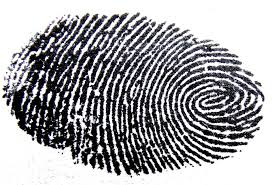
\includegraphics[width=\linewidth]{fig/fingerprint.jpeg}
\end{columns}
\end{block}
\end{frame}

\begin{frame}{Benchmark Fingerprinting}
\begin{block}{Solution in our Reference Implementation (GBD)}
\begin{columns}
\column{.6\linewidth}
\begin{itemize}
\item Removal of comments and additional whitespace
\item Normalization of new-line characters
\item md5sum (integration)
\end{itemize}
\column{.3\linewidth}
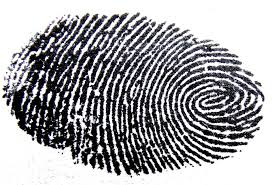
\includegraphics[width=\linewidth]{fig/fingerprint.jpeg}
\end{columns}
\end{block}
\end{frame}

\begin{frame}{Benchmark Fingerprinting -- Further Ideas}
\begin{block}{For Discussion: Increased Dedication, Loss of Integration}
\begin{itemize}
\item Hash Dimacs without the header (header information can be incorrect)
\item Improve Collision Avoidance by Appending e.g. ``Number of Variables''
\item Use other hash-function (sha-1)
\item Develop DIMACS-specific hash-function \dots 
\item \dots with invariance guarantees (e.g. w.r.t. clause order)
\end{itemize}
\end{block}
\end{frame}

\section{Reference Implementation -- Global Benchmark Database (GBD)}

\begin{frame}{Global Benchmark Database: GBD}
\begin{block}{Reference Implementation GBD}
\begin{itemize}
\item based on Python and SQLite
\item uses a two-column hash/value table for each attribute 
\item uses attribute types \emph{integer}, \emph{text}, \emph{double}
\item distinguishes ``unique'' and ``non-unique'' attributes
\item possibilty to specify a (queryable) default-value for certain attributes
\item pipe-based: query for hash value and pipe them to other gbd commands
\item automatic bootstrapping: initializes a table containing hashes and paths to locally available problems (local path is just another attribute)
\end{itemize}
\end{block}
\end{frame}

\begin{frame}{GBD -- Future Work}
\begin{itemize}
\item Continue to provide a reference implementation for the specification of a commonly used hash-function
\item include a REST webservice, easily expose database in the web and run queries against public URLs
\item Will be used to aggregate all the results of my thesis
\item Automatic import of header comments (specification of format)
\end{itemize}
\end{frame}

\section{Presentation}
\begin{frame}{Tool Presentation}
\begin{block}{GBD is maintained and available at}
\url{https://github.com/Udopia/gbd}
\end{block}
\end{frame}


\end{document}
